\documentclass{notes}
\usepackage[makeroom]{cancel}

\author{Ritchie Cai, Matthew Mosley \& Corey Higgins}
\title{Inverted Pendulum Summary}

\begin{document}
\maketitle 
\section{Introduction}
Our project is to simulate and implement an Inverted Pendulum (IP) system on Lego Mindstorm EV3 hardware.
Our modeling of the system is shown in figure~\ref{fig:system_simulation}(a). And the model we use
to implement the IP is shown in ~\ref{fig:system_simulation}(b). 

% For the past few weeks, we have been designing a system that consists of an inverted pendulum on two wheels. This design was constructed using the programmable BRIC from a LEGO Mindstorms EV3 set and additional LEGO pieces to physically construct it (seen in photos from modeling document). The overall goal of the system is to have the two wheels balance the pendulum in an upright, vertical position and to continue doing so after any slight disturbances that may offset the inverted pendulum by a relatively small angle (this assumed small angle comes into play in design calculations). 

\begin{figure}[h]
  \begin{center}
    \begin{minipage}[b]{1.5in}
      \mbox{\includegraphics[width=1.5in]{pics/Full_System_2.eps}}
      \mbox{\emph{(a)}}
    \end{minipage}
    \begin{minipage}[b]{1in}
      \mbox{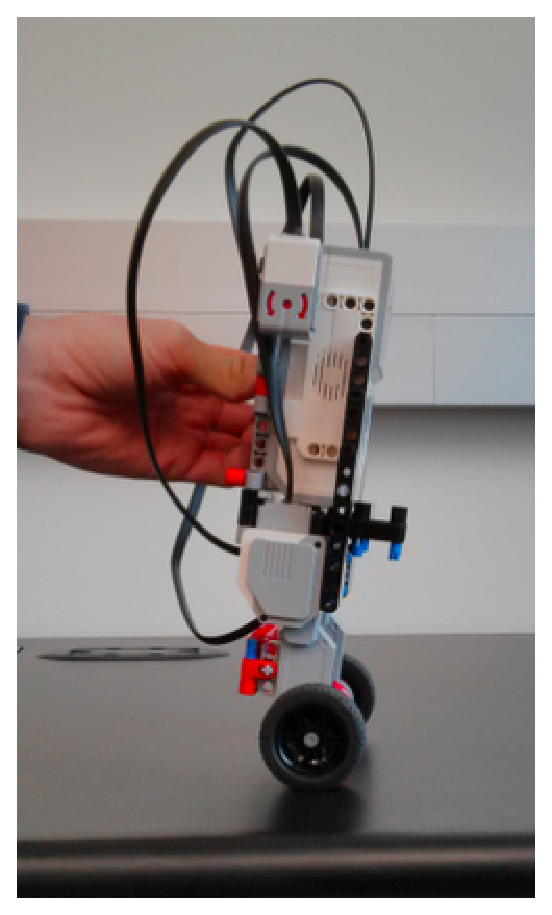
\includegraphics[width=1in]{pics/Lego/Build_side2.eps}}
      \mbox{\emph{(b)}}
    \end{minipage}
  \end{center}
  \caption{Inverted Pendulum System}
  \label{fig:system_simulation}
\end{figure}
\FloatBarrier

% \begin{figure}[!h]
%   \begin{center}
%     \includegraphics[width=2 in]{pics/Full_System_2.eps}
%   \end{center}
%   \caption{System setup for inverted pendulum}
%   \label{fig:system_simulation}
% \end{figure}

\section{Specifications}
The goal of the system is to make the pendulum stay at upright position, not falling down, by move
the pendulum's base back and forth when necessary. The only meaningful number we can give out is the
desired angle for the pendulum, which is 0 degree. Due to the fact that we have linearized our model from a
nonlinear model, system can only work for small angles. Which means when the pendulum lean too much,
our model will be extremely inaccurate. Thus we have to make sure our system output's rise time
to be as small as possible, oscillation is allowed as long as it eventually settles.


\section{Simulation}
In order to have an relative accurate simulation, we need to define a mathematical model for our
IP system. In our simulation we assume the pendulum is straight and its mass is evenly distributed.
By decomposing both centripetal and tangential acceleration of the pendulum body we are able to come
up with a transfer function that describe how the pendulum body reacts when given a acceleration on
it's base.

\[
  T(s) = \dfrac{\Theta}{U} = \dfrac{M+m}{m}\dfrac{\frac{2}{L}}{s^2-\frac{2g}{L}}
\]

We have decided to use PID controller to control our model. Feedback function is just 1, assuming
our gyro sensor will measure the correct angle. With guessing and experimenting, we found a set of
parameters that can make our pendulum system stable 1.2 after given an impulse input.

\section{Implementation}

The system is implemented on a Lego Mindstorm EV3 running LeJOS as it's operating system. Algorithms
are coded in Java. The effect of our modeled transfer function is now the real physics, giving an
acceleration to the base of the pendulum, we should have an change of angle. So the real challenge
here is to tune to PID controller to a state that come make the pendulum staying upright. 

We have tried Ziegler–Nichols method, which start with tuning $K_p$, and a different method that
start with tuning $K_d$. With the second method, the system have come to a state very close to
oscillating around center position. But due to time constrain and lack of experience we were unable
to find a suitable parameters.

\section{Failure Analysis}

There are many reasons we could not find the parameters. Time constrain and lack of experience
probably do count for quite a bit, but I also think there could some design issues. The main
processor unit of the Lego is quite heavy, and it's placed quite high relative to the wheels. So the
center of gravity is very high. This make the system very sensitive, thus require fairly precise set
of parameters in order to be stable. Also, our input acceleration is in terms of wheels' rotation.
But what really counts is the acceleration on horizontal axis which depending on the radius of the
wheels. Thus, with a design having lower center of gravity and larger wheels can probably make the
parameters much easier to find.

% The implementation of our controller is written in Java running on top of LeJOS which is a variance of the embedded Linux running embedded JVM. The Java interface allows us to control motors' acceleration and speed. In addition to motor we also have two gyro sensors, one is used to measuring the incline angle of the pendulum, the other one is used to measure the rate of change of the incline angle. The sensors prove to be a critical aspect of how we approached the math in the next section. Since we have control over acceleration and velocity of the motors driving the wheels, we would have to implement a design with an acceleration input. Then, our only way of effectively measuring the changing angle of the pendulum was through use of the two gyro sensors. So the angle would be our only output of our system in our design.

% \section{Analysis}  
% The designing process began with observing and analyzing the physics behind our system. Friction was ignored as the design intended to use a PID controller to cancel out friction's effect. For ease of calculation, we approximated our pendulum offset angles to be very small where sin($\theta$)= $\theta$, and cos($\theta$)= 1. As seen in the modeling document, we were able to derive the governing equations of motion behind our design. As expected, we observed that our inverted pendulum transfer function was unstable, which is clearly indicated by a pole existing in the positive, right half plane in our pole-zero diagram on the modeling document. This result made a controlling mechanism a necessity in order to gain stability for our system. As for the controller used, a simple PID controller was chosen along with negative feedback through the use of a LEGO Mindstorms EV3 gyro sensor. The unstable transfer function that represents the inverted pendulum system is as follows:
% \[
%   T(s) = \dfrac{\Theta}{U} = \dfrac{M+m}{m}\dfrac{\frac{2}{L}}{s^2-\frac{2g}{L}}
% \]
% This  transfer was then incorporated into the block diagram and then the transfer function that governed the entire system is represented by:

% Then the overall block diagram with negative feedback from gyro sensor looks like:
% \begin{figure}[!h]
%   \begin{center}
%     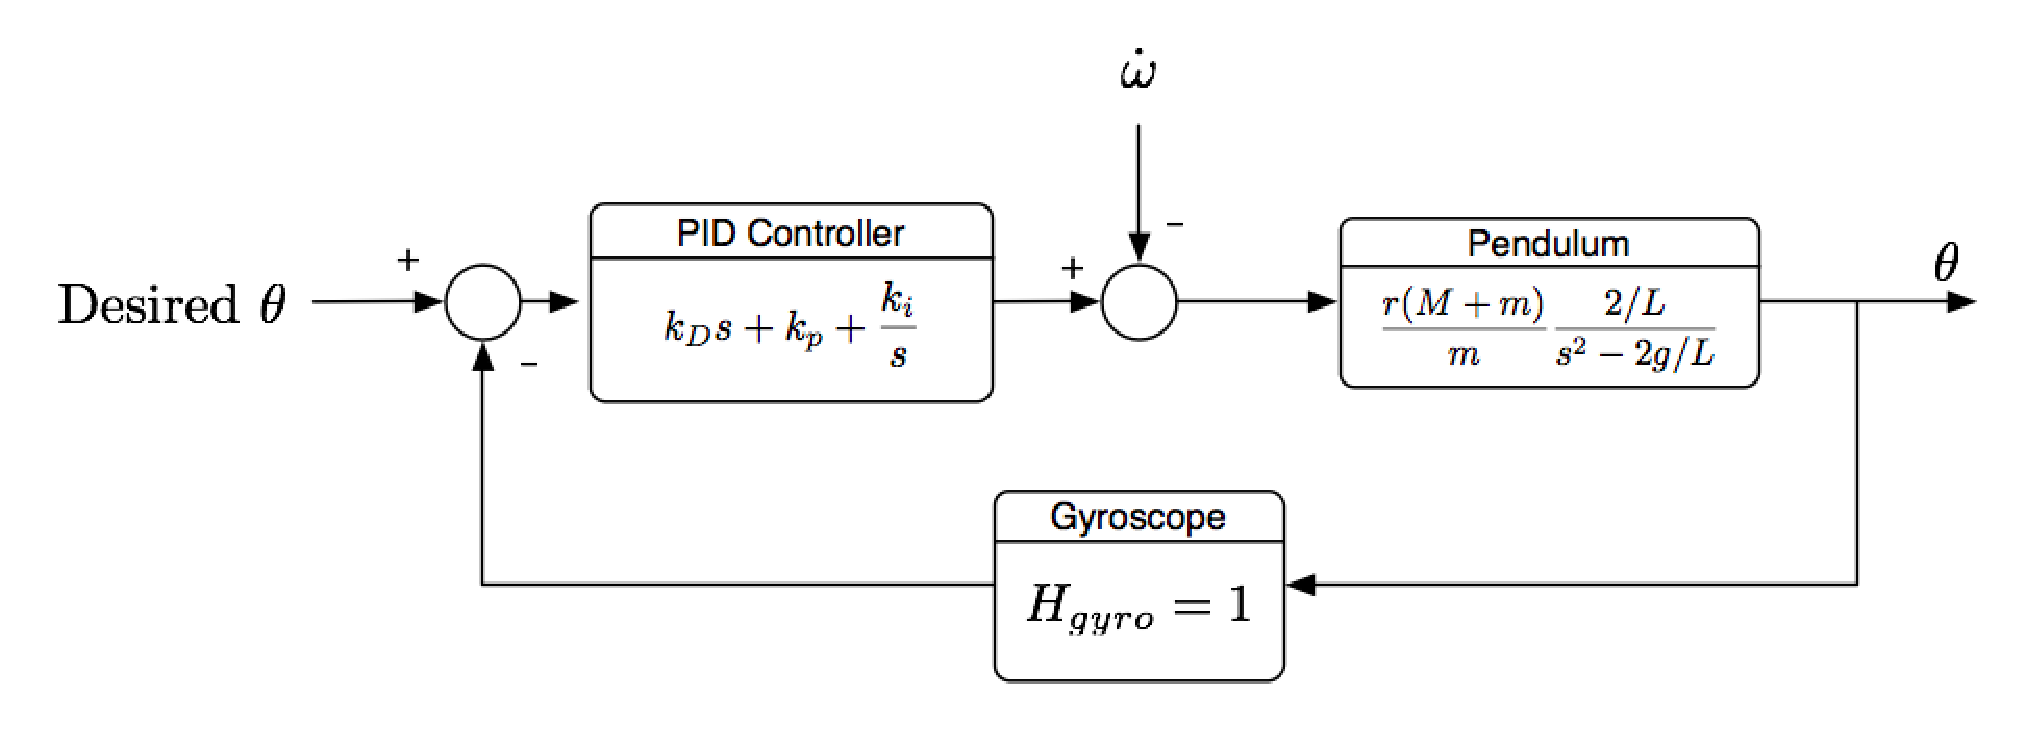
\includegraphics[width=5 in]{pics/Block_Diagram_2.eps}
%   \end{center}
%   \caption{Block diagram for our system}
%   \label{fig:block_diagram}
% \end{figure}

% \section{Design Specifications}
% We then went on to tune our system's parameters, $K_p$, $K_i$, and $K_d$, to optimize correction to any disturbance. In fact, the overall settling time simulated on MATLAB came out be 1.22 seconds. 
% The first transfer function can be described as having acceleration inputs and an angle theta, for the pendulum position, being the observed output. The design should adhere to the following specifications: settling time should be very responsive, pendulum angle theta never rotating beyond 20 degrees or so, and the steady state error should be small as well.  

%  \section{Results}
% The most difficult part of the design procedure was
   
\end{document}